% Template for PLoS
% Version 1.0 January 2009
%
% To compile to pdf, run:
% latex plos.template
% bibtex plos.template
% latex plos.template
% latex plos.template
% dvipdf plos.template

\documentclass[10pt]{article}

% amsmath package, useful for mathematical formulas
\usepackage{amsmath}
% amssymb package, useful for mathematical symbols
\usepackage{amssymb}

% graphicx package, useful for including eps and pdf graphics
% include graphics with the command \includegraphics
\usepackage{graphicx}

% cite package, to clean up citations in the main text. Do not remove.
\usepackage{cite}

\usepackage{color} 

% Use doublespacing - comment out for single spacing
%\usepackage{setspace} 
%\doublespacing


% Text layout
\topmargin 0.0cm
\oddsidemargin 0.5cm
\evensidemargin 0.5cm
\textwidth 16cm 
\textheight 21cm

% Bold the 'Figure #' in the caption and separate it with a period
% Captions will be left justified
\usepackage[labelfont=bf,labelsep=period,justification=raggedright]{caption}

% Use the PLoS provided bibtex style
\bibliographystyle{plos2009}

% Remove brackets from numbering in List of References
\makeatletter
\renewcommand{\@biblabel}[1]{\quad#1.}
\makeatother


% Leave date blank
\date{}

\pagestyle{myheadings}
%% ** EDIT HERE **


%% ** EDIT HERE **
%% PLEASE INCLUDE ALL MACROS BELOW

%% END MACROS SECTION

\begin{document}

% Title must be 150 characters or less
\begin{flushleft}
{\Large
\textbf{How to Eliminate the Unnecessary So That The Necessary May Speak? Biological Reference Points.}
}
% Insert Author names, affiliations and corresponding author email.
\\
Laurence T. Kell$^{1,\ast}$, 
Paul De Bruyn$^{2}$, 
Finlay Scott$^{3}$
Richard D.M. Nash$^{4}$
\\
\bf{1}  ICCAT Secretariat, C/Coraz\'{o}n de Mar\'{\i}a, 8. 28002 Madrid, Spain.
\\
\bf{2}  AZTI Tecnalia. Herrera kaia portualdea z/g, 20110 Pasaia, Gipuzkoa, Spain
\\
\bf{3}  The Fisheries Laboratory, Lowestoft, NR33 0HT, Suffolk, England
\\
\bf{4}  Institute of Marine Research, PO Box 1870 Nordnes, 5817 Bergen, Norway
\\
$\ast$ E-mail: Corresponding Laurie.Kell@iccat.int
\end{flushleft}

% Please keep the abstract between 250 and 300 words
\section*{Abstract}

% Please keep the Author Summary between 150 and 200 words
% Use first person. PLoS ONE authors please skip this step. 
% Author Summary not valid for PLoS ONE submissions.   
\section*{Author Summary}

\section*{Introduction}

%The ability to simplify means to eliminate the unnecessary so that the necessary may speak.  ~Hans Hofmann, Introduction to the Bootstrap, 1993

The adoption of the Precautionary Approach to fisheries management (FAO, 1996) requires a formal consideration of uncertainty. An important principle 
of the approach is that the level of precaution  should increase as uncertainty increases, e.g. from data rich to poor situations. However, defining stocks
as data rich or data poor based purely on the availability of catch and effort data obscures the fact that considerable uncertainty often exists about the 
biological processes of commercially important fish stocks. Examples include natural mortality, recruitment processes and stock structure. 
Conversely even when data are limited empirical studies have shown that life history parameters 
such as age at first reproduction, natural mortality, and growth rate are strongly correlated. Therefore biological knoweledge is important both
for evaluating the robustness of advice obtained from data-rich stock assessments and in allowing general rules, for example about choice of reference points, 
to be derived for all stocks.

Key questions for fisheries management are to identify the relative importance of the underlying biological assumptions made in stock assessment 
with respect to measures of interest and in achieving management objectives and how to prioritise research in order to reduce uncertainty.
For example, does uncertainty about the stock recruitment relationship have a relatively bigger effect than uncertainty about natural mortality 
on yield and sustainability? Elasticity analysis has  proved to be a useful tool in a number of areas of 
population and conservation biology, for example relating changes in vital rates to changes in the population life history \cite{grant2003density}
and to quantities of importance in management such as population viability \cite{heppell1998application}.  

Elasticity analysis is different to a sensitivity analsysis. A sensitivity analysis quantifties the effect of changing assumptions, for example 
what is the difference between estimates of MSY assuming that M is 0.2 or that M declines with age as indicated by life history theory.
While elasticity analysis evalutes the relative importance of the assumptions within the current model structure, i.e. does changing
M result in a bigger relative change in MSY than changing the steepness of the stock recruitment relationship.

A fuller consideration of uncertainty within fisheries advice frameworks requires for example Bayesian approaches or Managemement Strategy Evaluation (MSE).
MSE is comminly used to evaluate the impact of different managed measures,  given a broad range of uncertainty. However
performing an MSE is a costly process in human resources and can take several years. Therefore, tools such as elasticity analysis, which
is comparatively less demanding to carry out, are important to 
help identify andd focus research and management efforts. For example, is it more important to reduce uncertainty about the stock 
recruitment relationship or natural mortality or to develop harvest control rules that are robust to such uncertainty? Elasticity analyses can 
be used to answer such questions and priotise research effort. It can also shift the current focus from defining stocks either as data poor or rich 
defined solely on fishery catch and effort towards a better understanding of biological processes. 

In this study we demonstrate how elasticity analsysis can be used for a generic study based on population dynamics based on life history theory.
We do this by first simulating a stock based on life history relationships \cite{gislason2008does} 
and then by projecting the stock from an unfished to 
an over-exploited state. We do this in order to compute elasticites to allow us to evaluate the relative importance of the different system or biological parameters
when assessing the stock relative to system characteristics defined by biological reference points. This allows us to address two important questions i.e. what is
the relative importance of the different biological processes in providing advice and and how robust is advice based on the common biological reference 
points.


% You may title this section "Methods" or "Models". 
% "Models" is not a valid title for PLoS ONE authors. However, PLoS ONE
% authors may use "Analysis" 
\section*{Materials and Methods}

Even when data are limited, empirical studies have shown that in teleosts there is significant correlation between the life history parameters  
such as age at first  reproduction, natural mortality, and growth rate \cite{roff1984evolution}.  While size-spectrum theory 
and multispecies models suggest that natural mortality scales with body size \cite{andersen2006asymptotic}, 
\cite{pope2006modelling} and \cite{gislason2008coexistence}. This means that from something that is easily observable like the maximum size 
it is possible to infer life history parameters that are not easily observable.

\cite{gislason2008does} summarised life history characteristics and the relationships between them for a range of stocks and species. 
These relationships were used to parameterise an age-structured population model using model describing growth, maturation and natural mortality.
This population was then projected for an increasing fishing mortality and the SSB and fishing mortality relative to $B_{MSY}$ and $F_{MSY}$
used as indices of stock status. The elasticities of these indices in each year relative to the parameters in model were then used to
evaluate the relative importance of the various processes (i.e. growth, maturation, stock recruitment, natural mortality and selectivity of the fishery)
and the parameterisation of those process (e.g. k the rate of growth and $L_{\infty}$ with respect to stock status. We compare estimates of stock status in absolute terms 
(e.g. SSB and biomass) and relative to refence points. The reference points considered were $F_{MSY}$, the level of exploitation that provides the maximum 
sustainable yield, a proxy for $F_{0.1}$ (the fishing 
mortality that corresponds to a point on the yield per recruit curve where the slope is 10\% of that at the origin) and  $F_{Crash}$ 
the level of F that will drive the stock to extinction. All depend upon the selection pattern,  
since not all ages are equally vulnerable to a fishery and if there is a refuge for older fish, a higher level of fishing effort will be sustainable.
Also if the fecundity of older fish is greater than the fecudity of younger fish of the same mass-at-age, e.g. due to maternal effects or repeat
spawners being more fecund then a condideration of the interactions between biology and selectivity will be important.

The analysis allows us to evaluate where more biological knowledge is needed and to identify robust reference points for use in management. Following this analysis
sensitivy analysis could be conducted to help quantify the costs and benefits and MSE to develop robust management advice.

\subsection{Life History Relationship}

The Russell equation \cite{russell1931some} summarises the key processes influencing the dynamics of exploited populations i.e.
 
\begin{equation}f(B) = (I-E) + G + R – (F+M)\end{equation}

where a biomass B is a function of the gains due immigration (I), growth (G) and recruitment (R) and the losses due to emigration (E), fishing (F) and natural 
mortality (M). The knowledge about these processes affects our ability to provide robust scientific advice. In this paper we concentrate 
on G,R,F \&M as we assume a single heterogenerous population with out emmigration or immigration; However our approach could easiliy be extended to include I \& M.

Life history relationship were used to parameterise approprite functional forms for the various processes in order to provide a generic framework for
modelling a variety of stock dymanics. This also allows processes to be modelled under a variety of assumptions and for the impact of the various parameters
to be evaluate.  

Parameterisation of the processes

\begin{description}
    \item[Growth] is modelled by the Von Bertalanffy growth equation \cite{von1957quantitative}

      \begin{equation} L_t = L_{\infty} - L_{\infty}exp(-kt) \end{equation}
         
where  K is the rate at which the rate of growth in length declines as length approaches $L_{\infty}$ 
the asymptotic length and $t_{0}$ is the time at which an individual is of zero length. 
Length is converted to mass using the condition factor (a) and allometric growth coefficient (b)

\begin{equation} W = a \times L^b \end{equation}

 \item[Recruitment] is split into Spawning Reproductive Potential (SRP) and the stock recruitment relationship (SRR).

SRP is the sum of the products of the numbers of females (n), proprtion mature-at-age (Q) and their mean gonadal mass-at-age (E), i.e. 

   \begin{equation} SRP = \sum{n \times Q \times E } \end{equation}

where their mean gonadal mass-at-age is equal to 
\begin{equation} E = a \times L^{b\prime} \end{equation}

if a and b as the same as in equation 3 then SRP is equivalent to female spawning stock biomss (SSB).

Proprtion mature is modelled by the logistic equation with 3 parameters, $\mu$ age at 50\% mature, age at 95\% mature and the asymptotic value asym. The 
latter allows SRP to not be equivalent to stock mass-at-age

\begin{equation}
f(x) = \left\{ \begin{array}{ll}
			0                                 &\mbox{ if $(a50-x)/ato95 >  5$} \\
			asym                              &\mbox{ if $(a50-x)/ato95 < -5$} \\
			\frac{asym}{1.0+19.0^{(a50-x)/ato95)}} &\mbox{ otherwise}
		\end{array}
       \right.
\end{equation}

Parameters can be derived as in Williams and Shetzer (2003) from the theoretical relationship between M, K, and age at maturity $a_{Q}$ 
based on the dimensionless ratio of length at maturity to asymptotic length \cite{beverton1992patterns}. Here we based it on the empirical relationship
between $L_{\infty}$ and age at maturity \cite{froese2000empirical} e.g.

\begin{equation}
  a50=exp^(0.8776 \times logl_{\infty}-0.038)
\end{equation}

We use a Beverton and Holt stock recruitment relationship reformulated in terms of steepness (h), virgin biomass (v) and $S/R_{F=0}$. 
Where steepness is the ratio of recruitment at 40\% of virgin biomass to recruitment at virgin biomass. However, steepness is difficult to estimate from 
stock assessment data sets and there is often insufficient range in biomass levels that is required for its estimation \cite{ISSF2011steep}.

Where steepness is the proportion of the expected recruitment produced by 20\% of virgin biomass relative to virgin recruitment $(R_0)$. For the BevertonHolt 
stock-recruit formulation

\begin{equation}
R=\frac{0.8 \times R_0 \times h \times S}{0.2 \times S/R_{F=0} \times R_0(1-h)+(h-0.2)S}
\end{equation} 

Steepness and virgin biomass were set a 0.9 and 1000 t respectively.

 \item[Natural mortality]  derived from the life history relationship \cite{gislason2008does}.
               
\begin{equation}
            M = exp(-2.11 -1.70log(L) + 1.51log(L_{\infty}) + 0.97log(k) + a[5]/T),
\end{equation} 
where $L$ is the average length of the fish (in cm) for which the M estimate applies.

 \item[Selection pattern] 

The selectivity of the fishery can be represented by a double normal 
(see Hilborn et al. 2001) with three parameters that describe the age at maximum selection (a1), the rate at which the lefthand 
       limb increases (sl) and the righthand limb decreases (sr) which allows flat topped or domed shaped selection patterns to be chosen.

Even in data poor situtations where catch-at-age for the entire catch time series is not available, some data will normally exist for 
some years or gears or for similar stocks and species. In cases where some length frequency data are available the shape of selection pattern, i.e.
age at recruitment to the fishery, can be estimated using a method like that of Powell-Wetherall \cite{wetherall1987estimating}. This allows
a double normal curve to be parameterised, i.e. age at maximum selectivity and whether the selection pattern is flat topped or dome shaped.



\begin{equation}
f(x) = \left\{ \begin{array}{rl}
 2^{-[(x-a_1)/s_L]^2} &\mbox{ if $x<a_1$} \\
 2^{-[(x-a_1)/s_R]^2} &\mbox{ otherwise}
       \end{array} \right.
\end{equation}
 

\end{description}


\subsection{Seasonality}

The model is a discrete population model where the number of individuals in a year-class in year is a function of the number of individuals in the previous year.
However, processes like growth, maturation, natural mortality and fishing occur in different seasons of the year. Therefore to take account of this the age for which
the expected values of mass, maturity and natural mortality-at-age can vary. 

For the stock mass-at-age lengths and mass are calculated at spawning time, catch mass-at-age is calculated in mid year and natural mortality is a function of the lengths-at-aged 
mid year.  

\subsection{Elasticity}

Elasticity is an important measure in economics of how changing a variable influences quantities of interest, e.g. if the price of an item 
changes how will this affect sales.
 
Mathematically the elasticity of y with respect to x is 

\begin{equation}
 E_{y,x} = \left| \frac{\partial \ln y}{\partial \ln x} \right|        
     = \left| \frac{\partial  y}{\partial  x} \cdot \frac{x}{y} \right|
       \approx \left| \frac{ \%\bigtriangleup  y}{\%\bigtriangleup x} \right|  
  \end{equation} 

The absolute value operator is used for simplicity although the elasticity can also be defined without the absolute value operator when the direction of 
change is important, e.g. to evaluate if a reduction in natural mortality increases or decreases MSY reference points.	


% Results and Discussion can be combined.
\section*{Results}

Reference points considered were MSY, $F_{0.1}$ (a proxy for MSY) and $F_{Crash}$ a limit reference point. $F_{0.1}$ is the fishing mortality on the yield per recruit
curve where the slope is 10\%  of that at the origin, a conservative proxy for $F_{MSY}$. $F_{Crash}$ is the fishing mortality that will drive the
stock to extinction since it is equivalent to a R/S greater than the slope at the origin of the stock recruitment relationship, i.e. recruitment can not replace removals
for a fishing mortality equal to $F_{Crash}$.  

Growth, proportion mature, natutural mortality and selectivity-at-age are shown in figure 1. While the expected or equilibrium dynamics, along with 
MSY, $F_{0.1}$ the $F_{MSY}$ proxy and limit reference point $F_{crash}$ are shown in figure 2. Based on these equilibrium dynamics a population was 
simulated at a range of fishing mortalities from 0 to $F_{Crash}$. These are plotted in figure 3 as a phase plot; where the x-axis corresponds to $biomass:B_{MSY}$ and the 
y-axis $harvest:F_{MSY}$. The red zone corresponds to a stock that is both over fished and where over fishing is occurring. Quadrants are defined for the 
stock amd fishing mortality relative to $B_{MSY}$ and $F_{MSY}$; i.e. red when $B<B_{MSY}$ and $F>F_{MSY}$, green if $B≥B_{MSY}$ and $F≤F_{MSY}$,
and yellow otherwise. I.e. the red quadrant refers to an overfished stock subject to overfishing, green to a stock which is neither overfished stock 
or subject to overfishing and the yellow to a stock which is one of either overfished stock or subject to overfishing.

Plots of elasticities with respect to process, parameter and fishing mortality are presented in figures 4,5,6 and 7, for SSB, fishing mortality, biomass and yield
relative to the three reference points. The vertical line indicates the boundary between the red and green quadrants and the horizontal line 0, i.e. where varying
a parameter has no effect.

These plot allows serveral important questions to be addressed, e.g, which processes and parameters have the biggest impact and are some reference points more 
robust to uncertainty in key processes than others. Also does this depend upon the stock status, i.e. is knowledge on some parameters and processes more
important when a stock is depleted than when it is within safe biological limits. Are F reference points for example more robust than those based on SSB.	

Inspection of the elasticites in plot 4 for SSB shows that the process that has the biggest relative effect on assessing the stock relative to the three
reference points in M and parameter M2, which determines the rate at which M declines with length. The next most important process is  stock recovery
and the assumed steepness. The other processes growth, maturity and selectivity have similar impacts to each other; the most important parameters are k,
age at 50\% mature and age at recruitment to the fishery for growth, maturity and selectivity respectively.
Next we compare the elasticites for stock above MSY (to the left of the vertical line); the elasticites 
for $F_{MSY}$ and $F_{0.1}$ are very similar with the values for $F_ {MSY}$ tending to be of smaller magnitude, i.e. MSY is more robust to uncertainty
than $F_{0.1}$.  The values for $F_{Crash}$ are on average greater than for the other two reference points. For a depleted stock (to the right of the line)
the elasticites for $F_{Crash}$ are generally lower in magnitude. In conclusion it appears that for SSB $F_{MSY}$ and $F_{0.1}$ are more robust target
reference points than  $F_{Crash}$, while the reverse is true for limit reference points.

Similar findings are found based for biomass in figure 6, expect that  $F_{Crash}$ elasticites are greater for stocks above $B_{MSY}$ and 
for yield in figure 7. 


Inspection of the elasticites in plot 4 for fishing mortality shows that elasticities do not vary by exploitation level and that M is much more
important that the stock recruitment relationship. While MSY appears to have lowest elasticites and so is the more robust reference point
for fishing mortality.
 
\section*{Discussion}


\begin{description}
 \item Relative importance of processes
 \item Robustness of refence points, Red v Green quadrant, also the points with the transiton periods
 \item Use of Gislason et al.'s mortality relationship more realistic than the common practice of using an M which does not vary with life history stage. 
Numerous studies on early life history mortality, highlight the Nash \& Geffen (2012) paper plaice moralties. 
\end{description}
    
\section{Conclusions}\label{Conclusions}

\begin{description}
 \item[What we did] Compared the relative importance of biological parameters when assessing stocks relative to target and limit reference points
 \item[What we found] That in general target reference points such as MSY and $F_{0.1}$ are more robust as limit reference points that actual limit reference points
                      such as $F_{Crash}$. The importance of processes and parameters depend upon stock status and current fishing mortality. 
                      This illustrates the importance of considering refence points not in isolation but as part of the design of HCRs. For example 
                      if you know that a parameter is highly uncertain then when chosing a target or lmit refence point then you should choose a 
                      reference point that is robust to such uncertainty, i.e. if you dont know the shape of the M curve use a multiple (e.g. 1.5) of $F0.1$ 
                      as a limit refence point instead of $F_{Crash}$ 
 \item[What we didn´t] The analsysis is limited in that it assumes a given model structure, i.e. exponentially declining M, SSB is an appropraite measure of SRP and
                       a Beverton and Holt SRR. There are two issues here a) we don´t actually know the correct functional form of M and SRR and b) we don´t
                       know whether advice based on TEP is better than than based on SSB.                         
 \item[Future work] BBNs \& MSE
\end{description}

% Do NOT remove this, even if you are not including acknowledgments
\section*{Acknowledgments}


%\section*{References}
% The bibtex filename
\newpage
\bibliography{refs} 

%\bibliography{template}

\section*{Figure Legends}

\begin{figure}[!ht]
\begin{center}
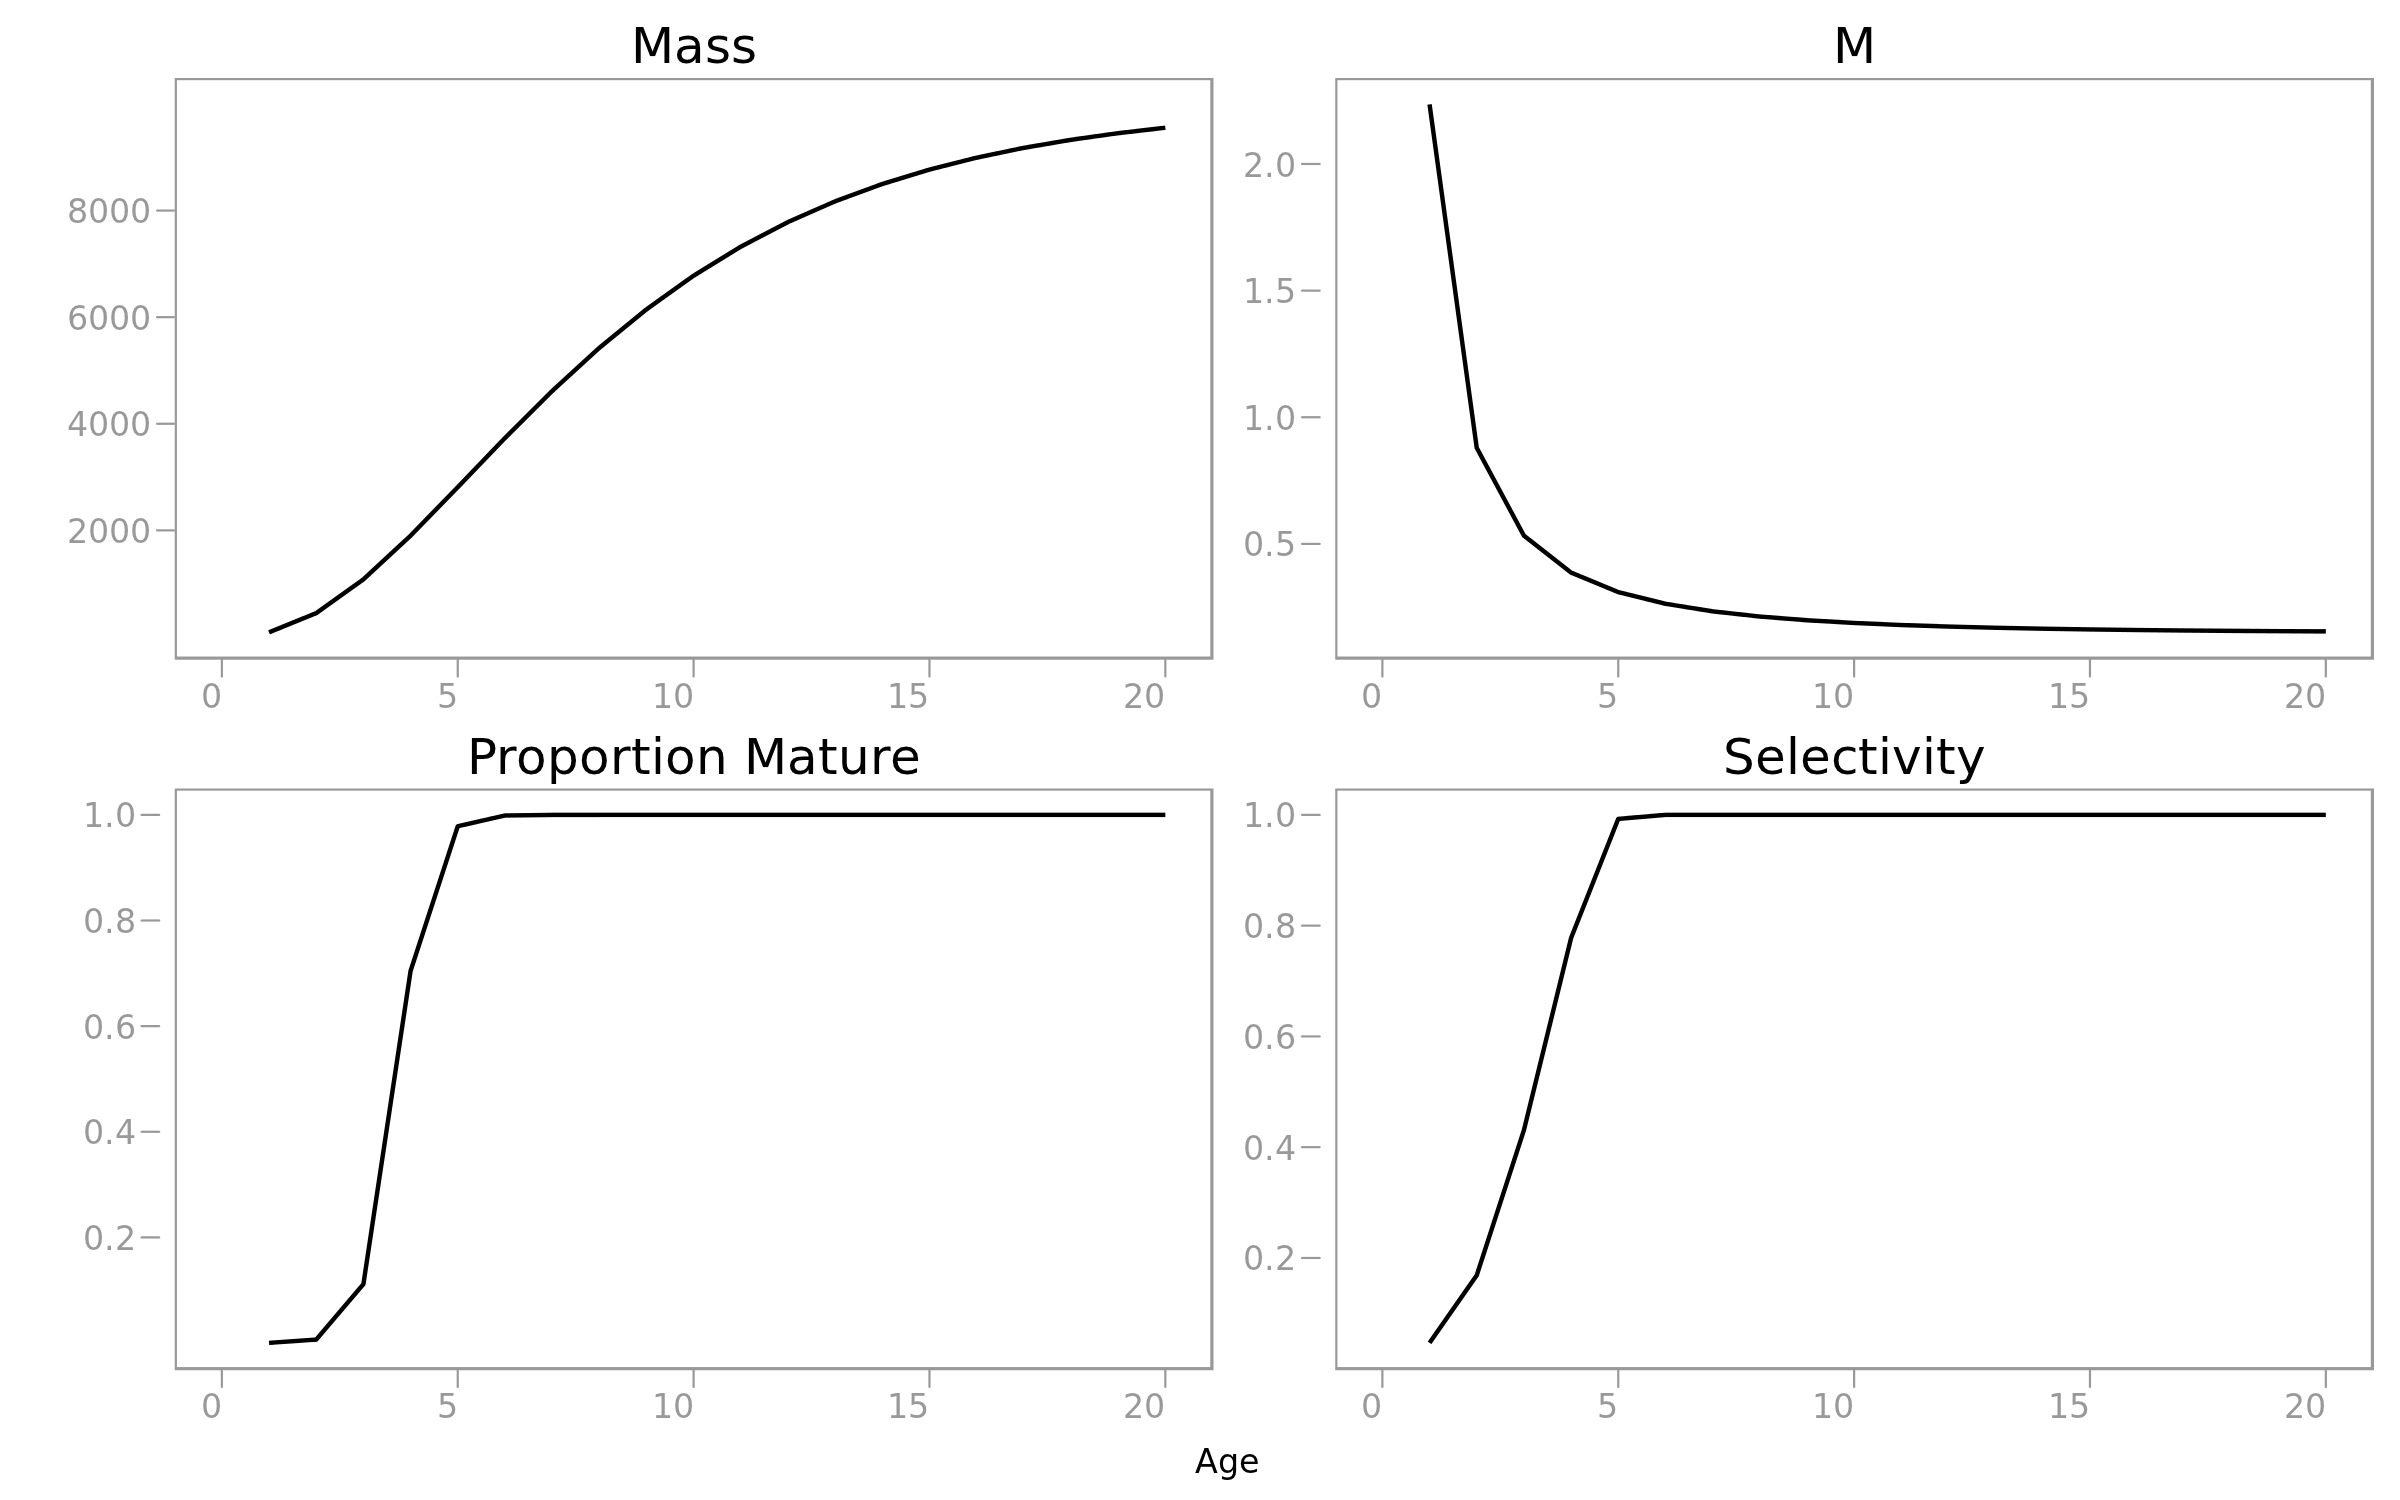
\includegraphics[height=4in, width=4in]{fig1.png}
\end{center}
\caption{\bf{Mass, natural mortality, proportion mature and selection pattern-at-age.}}
\label{Figure_label_1}
\end{figure}

\begin{figure}[!ht]
\begin{center}
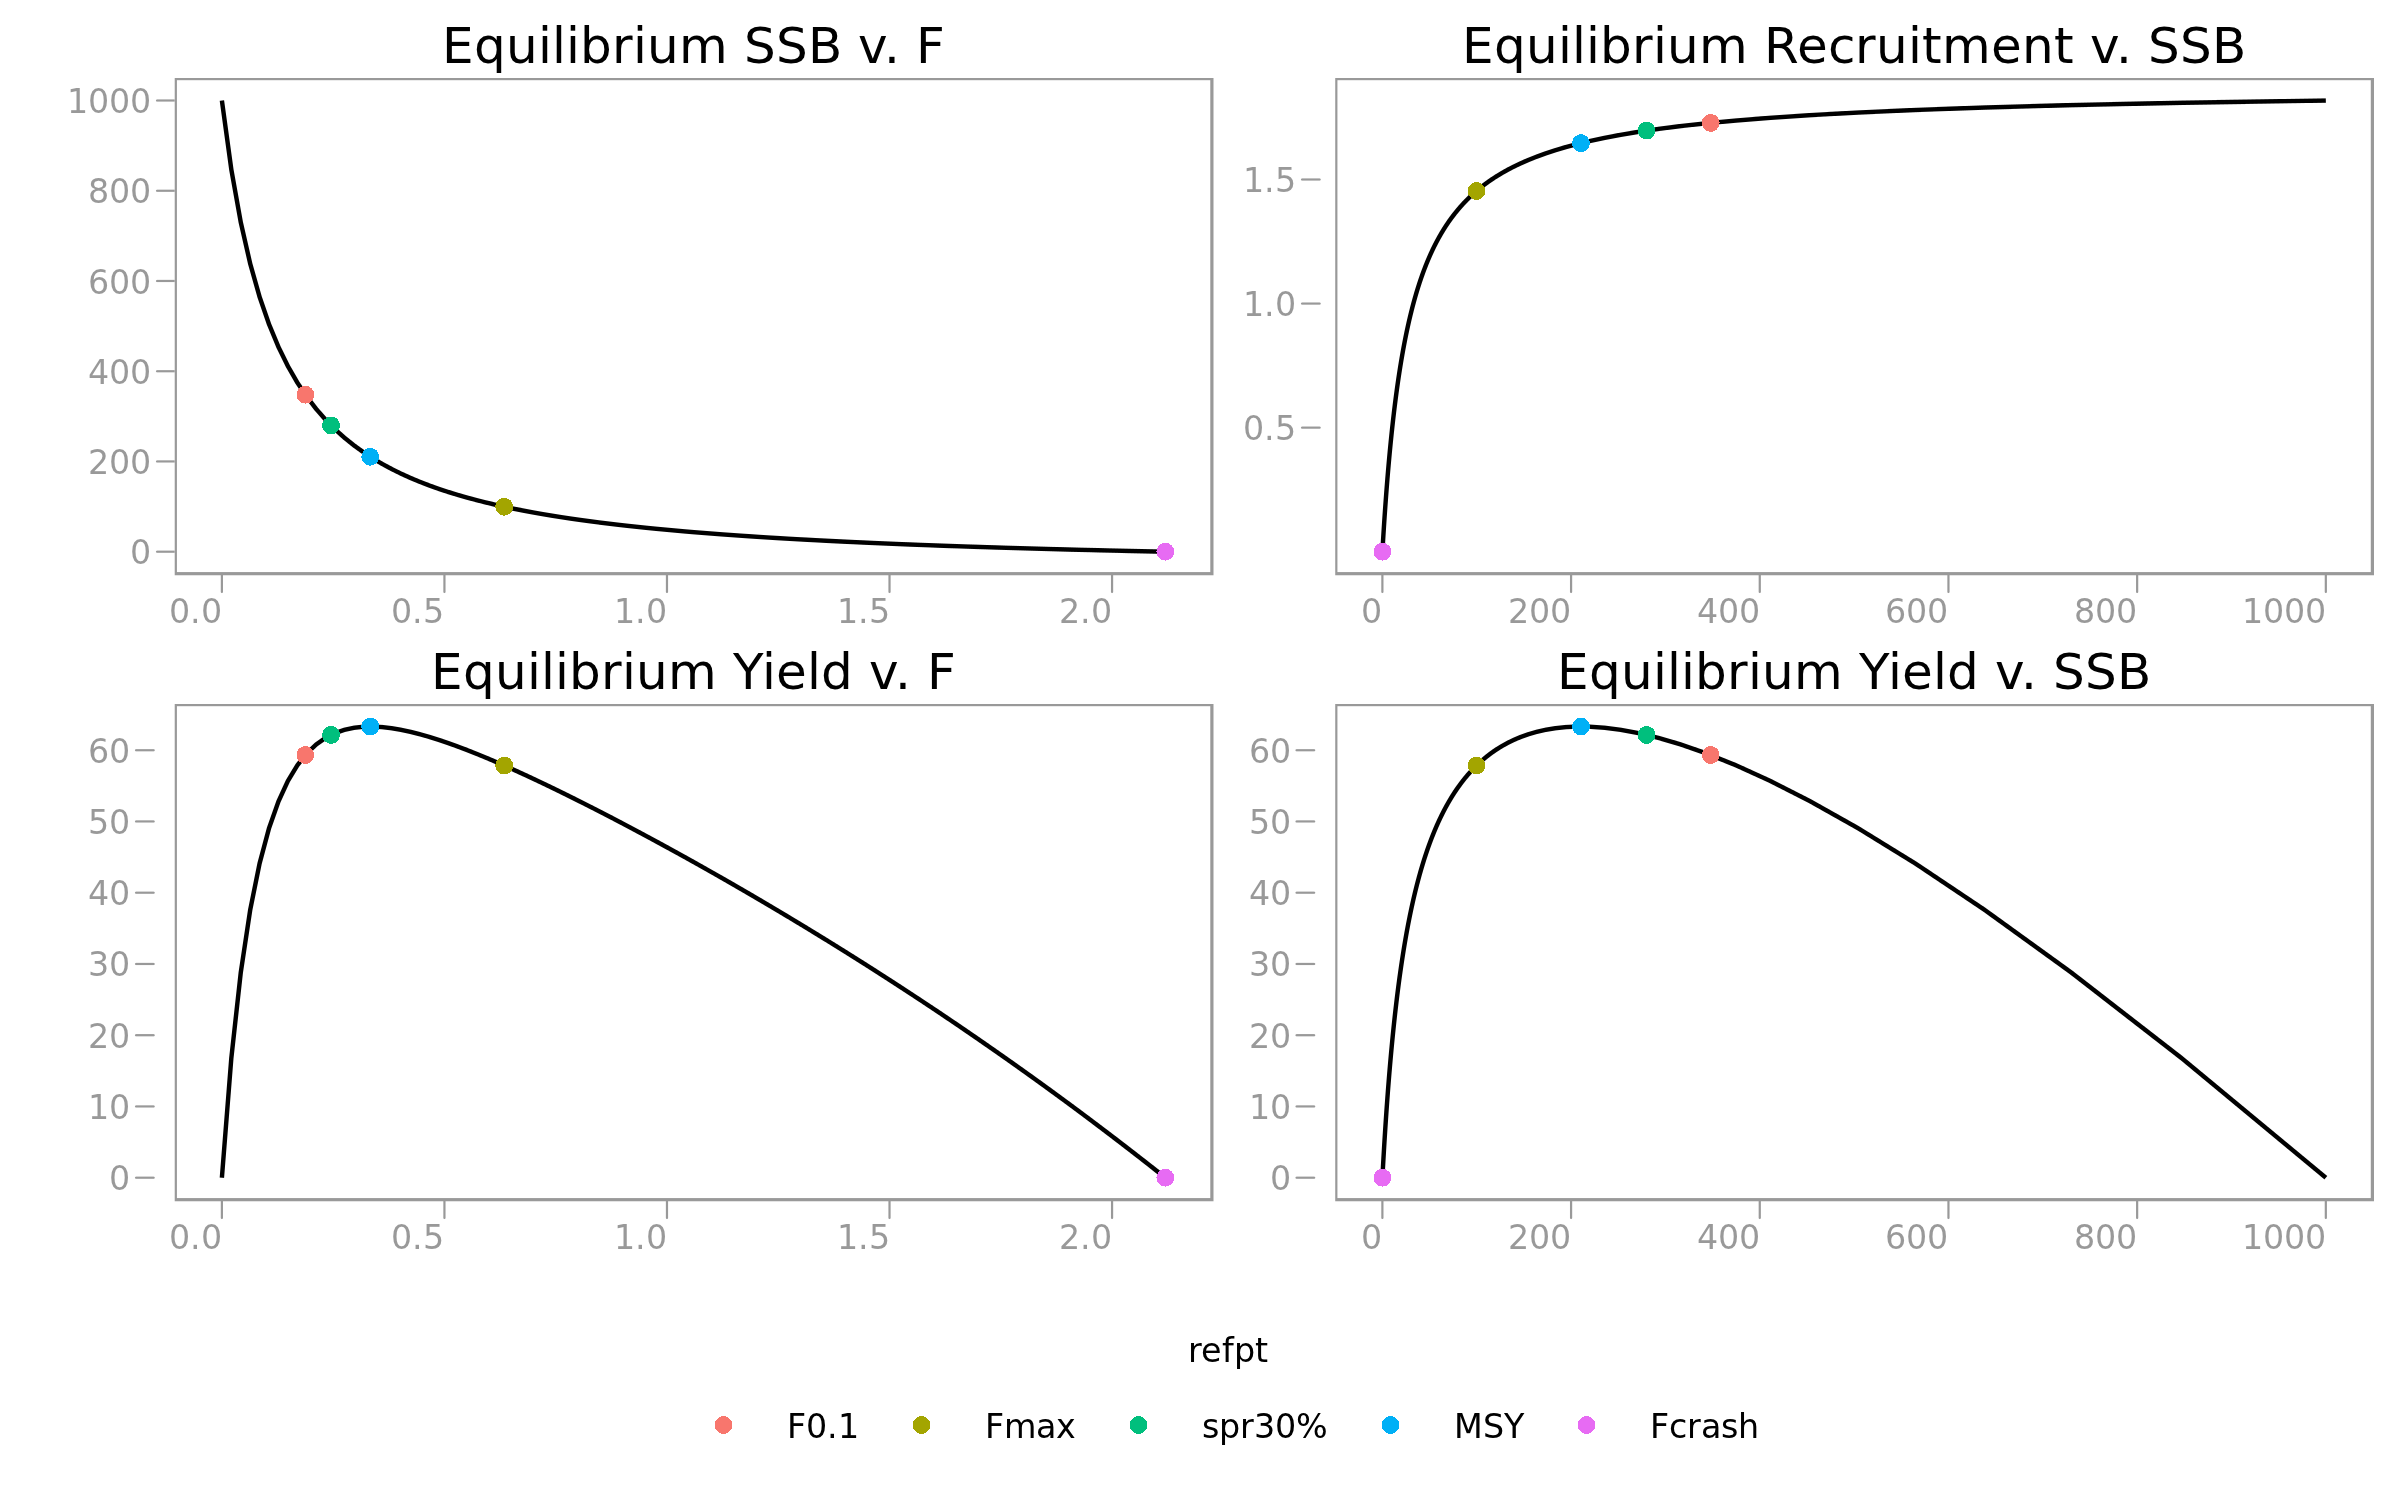
\includegraphics[height=2.1in, width=4in]{fig2.png}
\end{center}
\caption{\bf{Equilibrium (i.e. expected) values of SSB and yield verses fishing mortality and recruitment and yield verses SSB; points correspond to
MSY and MSY proxies ($F_{0.1}$, $F_{Max}$, SPR30\%) and limit ($F_{crash}$) reference points.}}
\label{Figure_label_2}
\end{figure}

\begin{figure}[!ht]
\begin{center}
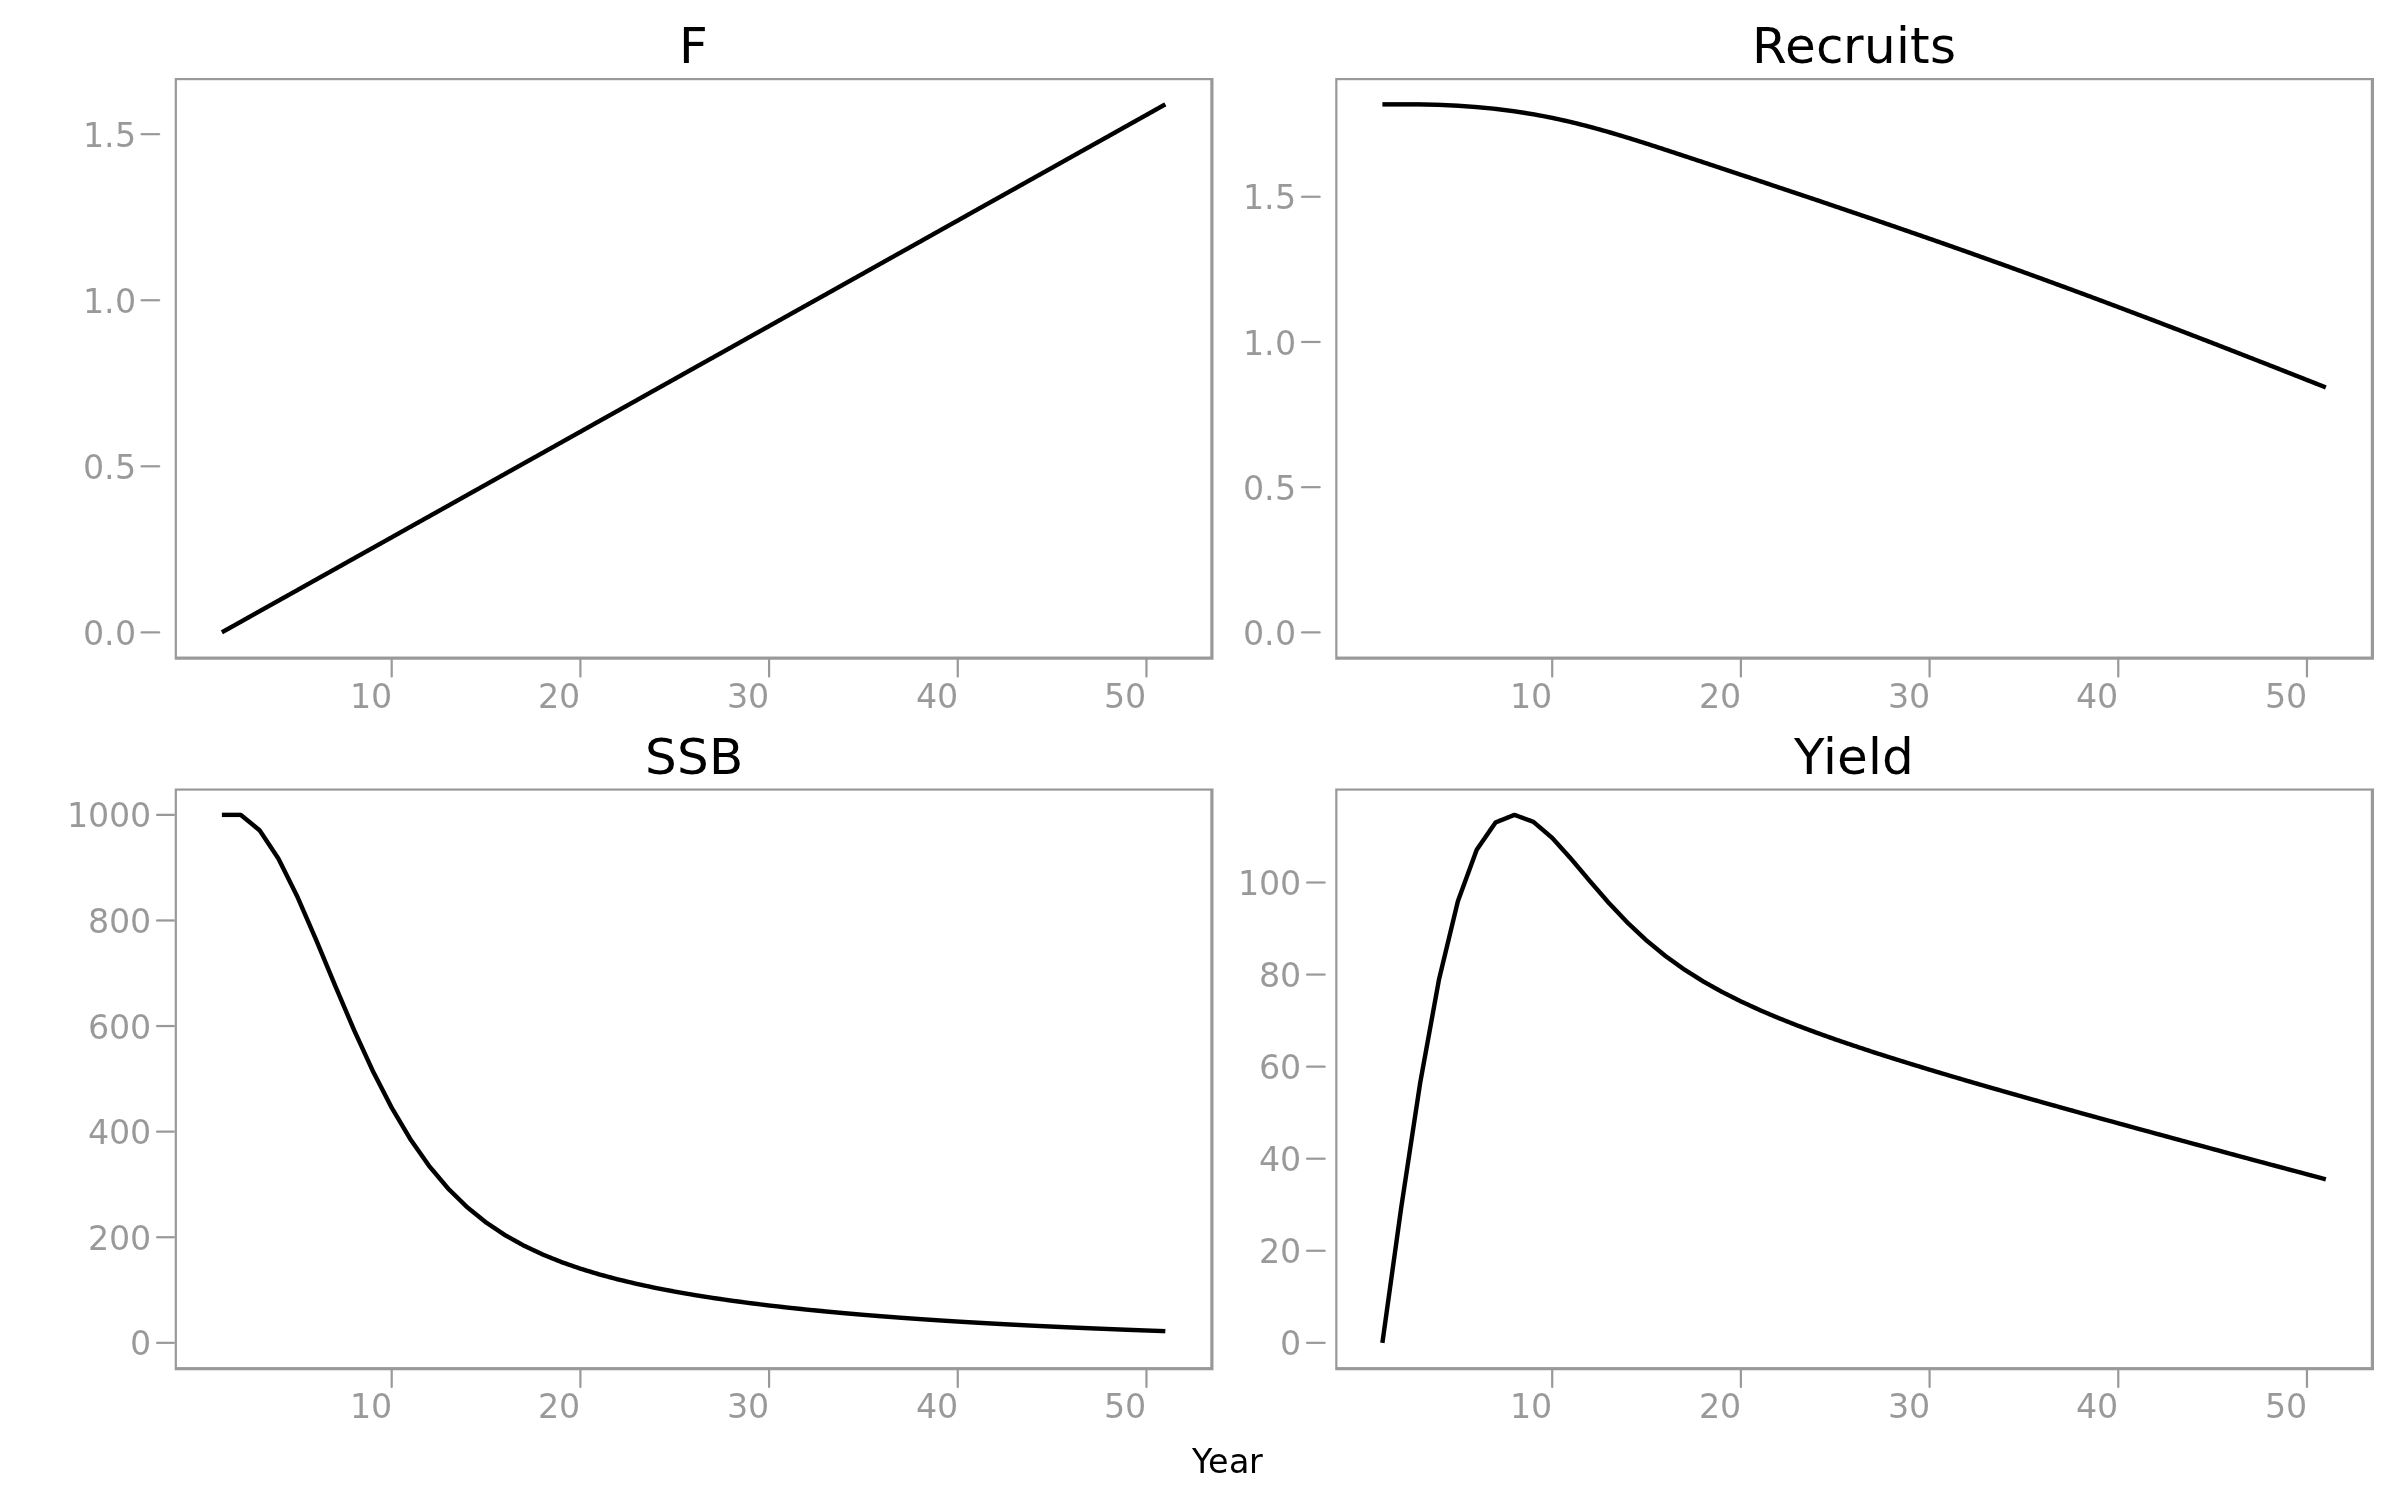
\includegraphics[height=2.1in, width=4in]{fig3.png}
\end{center}
\caption{\bf{Simulated trajectories of recruitment, SSB and yield for a increasing F.}}
\label{Figure_label_3}
\end{figure}

\begin{figure}[!ht]
\begin{center}
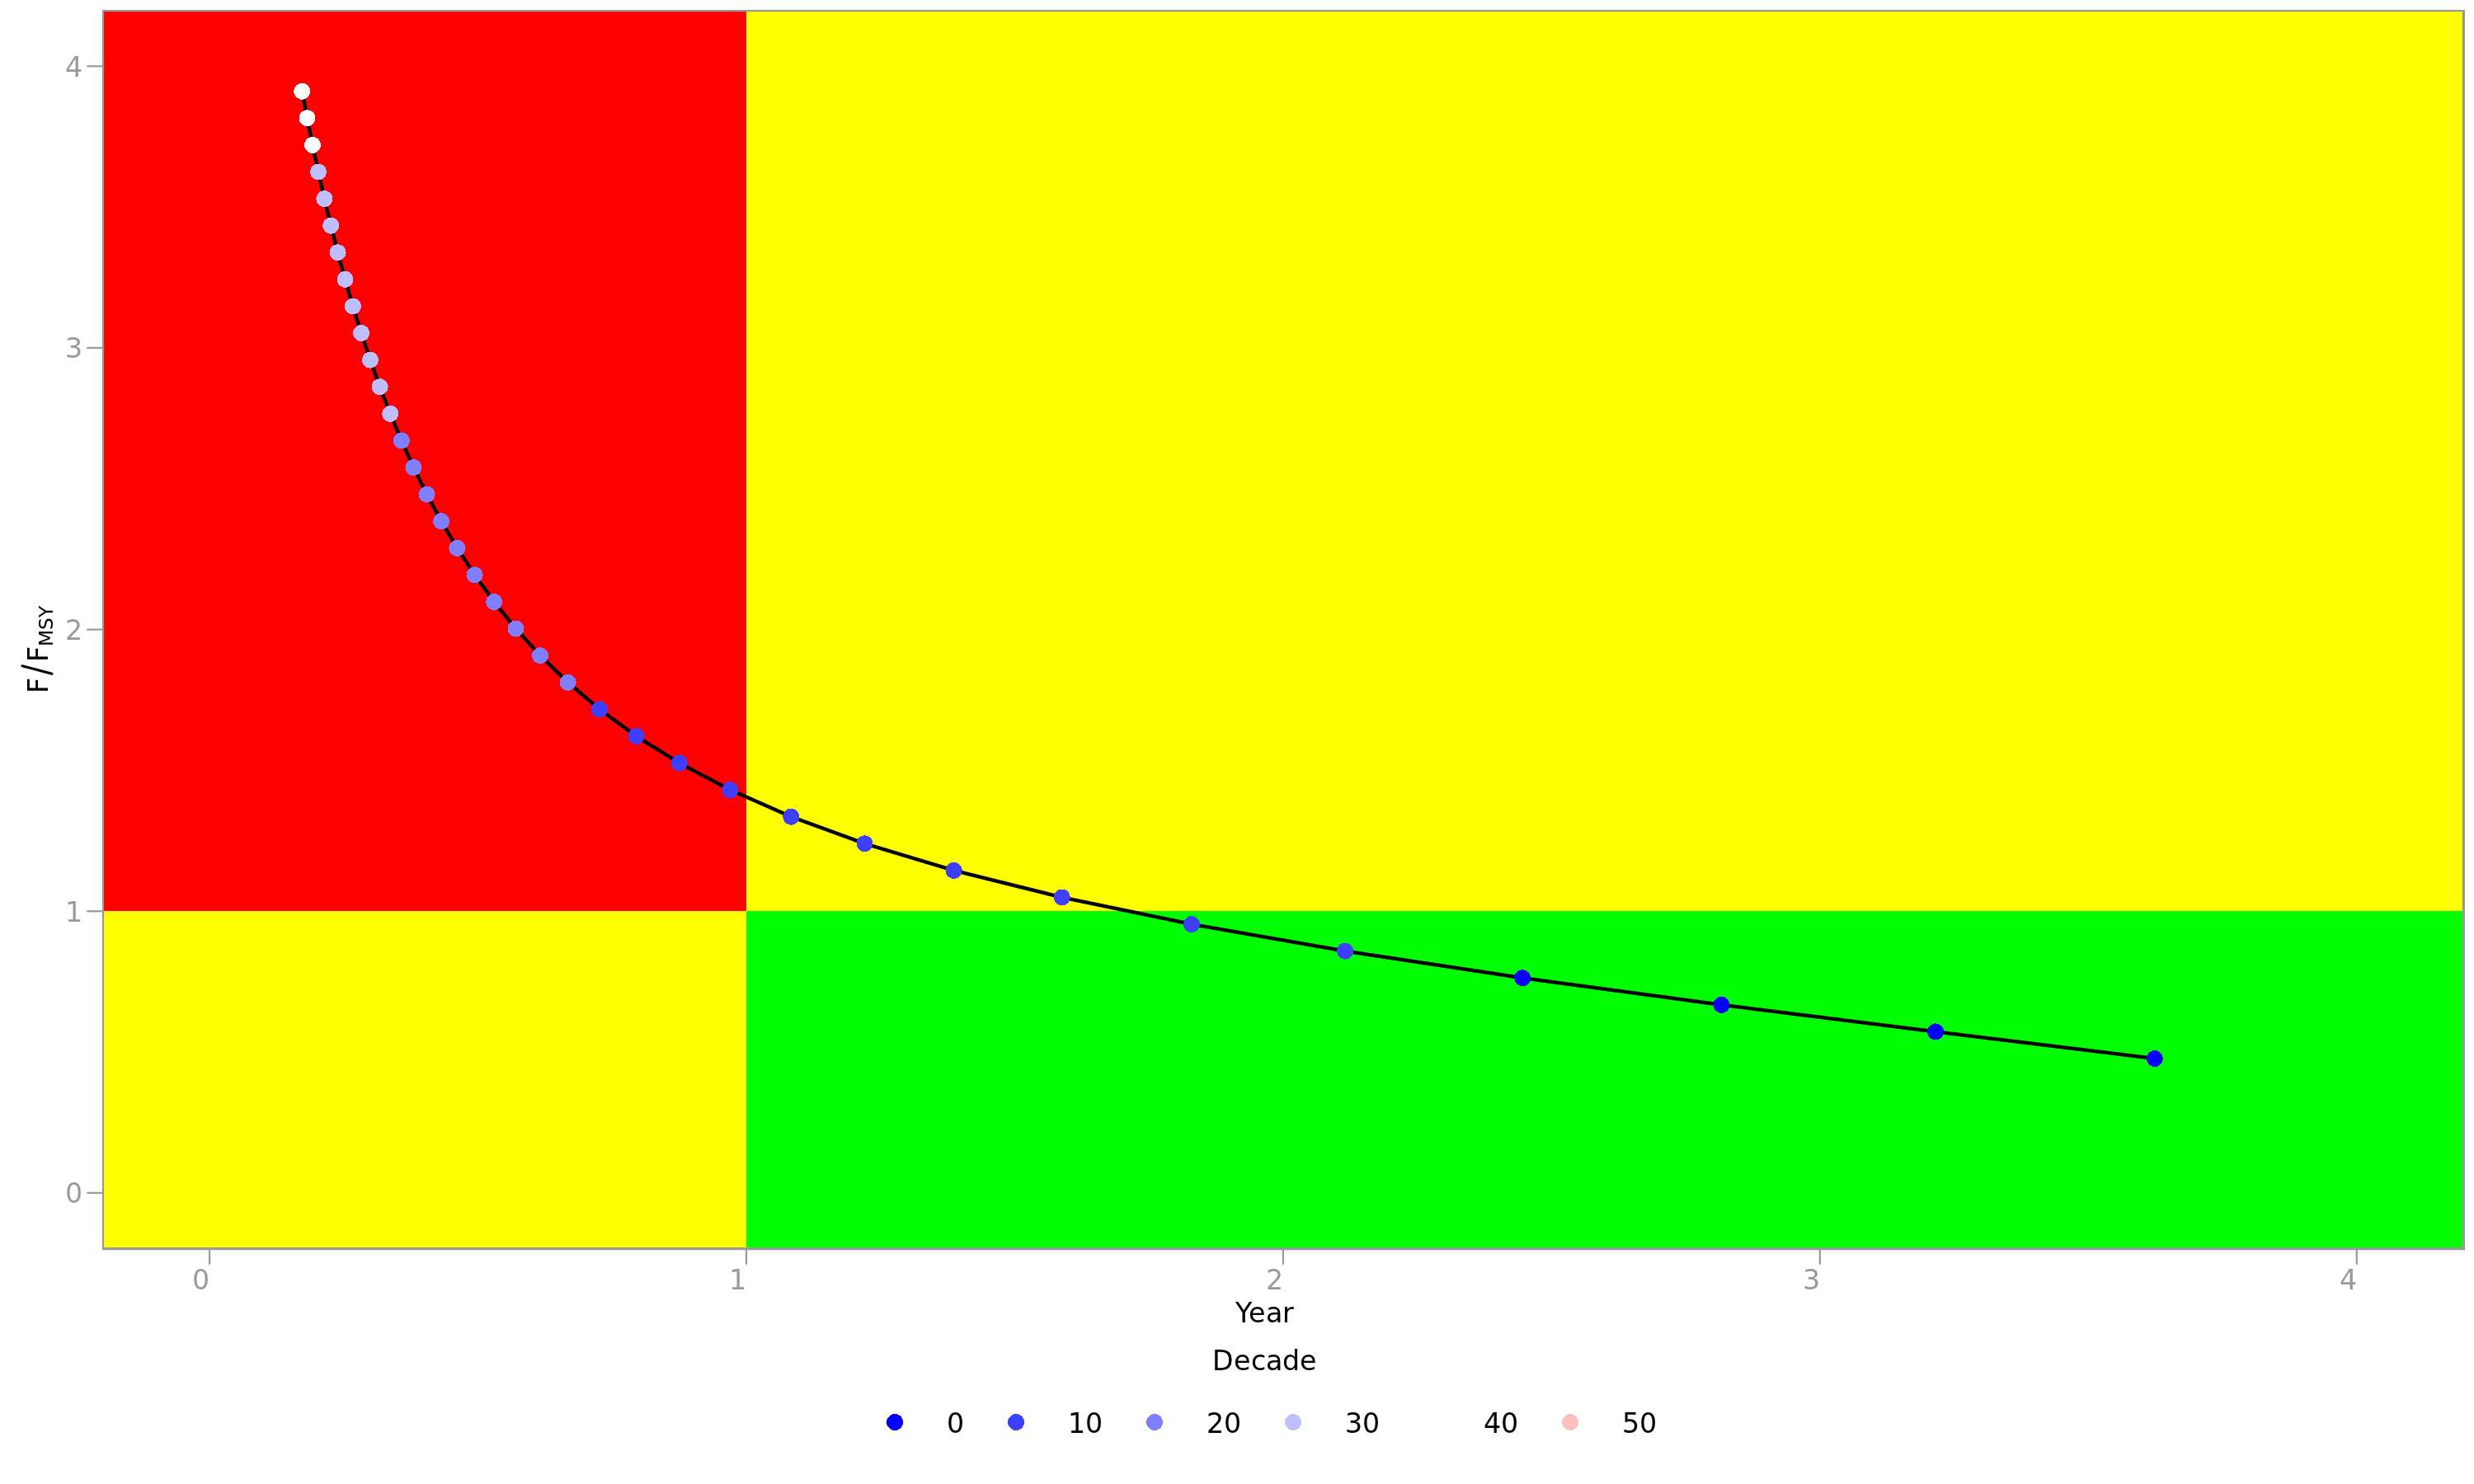
\includegraphics[height=4in, width=4in]{fig4.png}
\end{center}
\caption{\bf{Plots of elasticities for processess by year with respect to SSB for  MSY, $F_{0.1}$ and $F_{crash}$ reference points.}}
\label{Figure_label_4}
\end{figure}

\begin{figure}[!ht]
\begin{center}
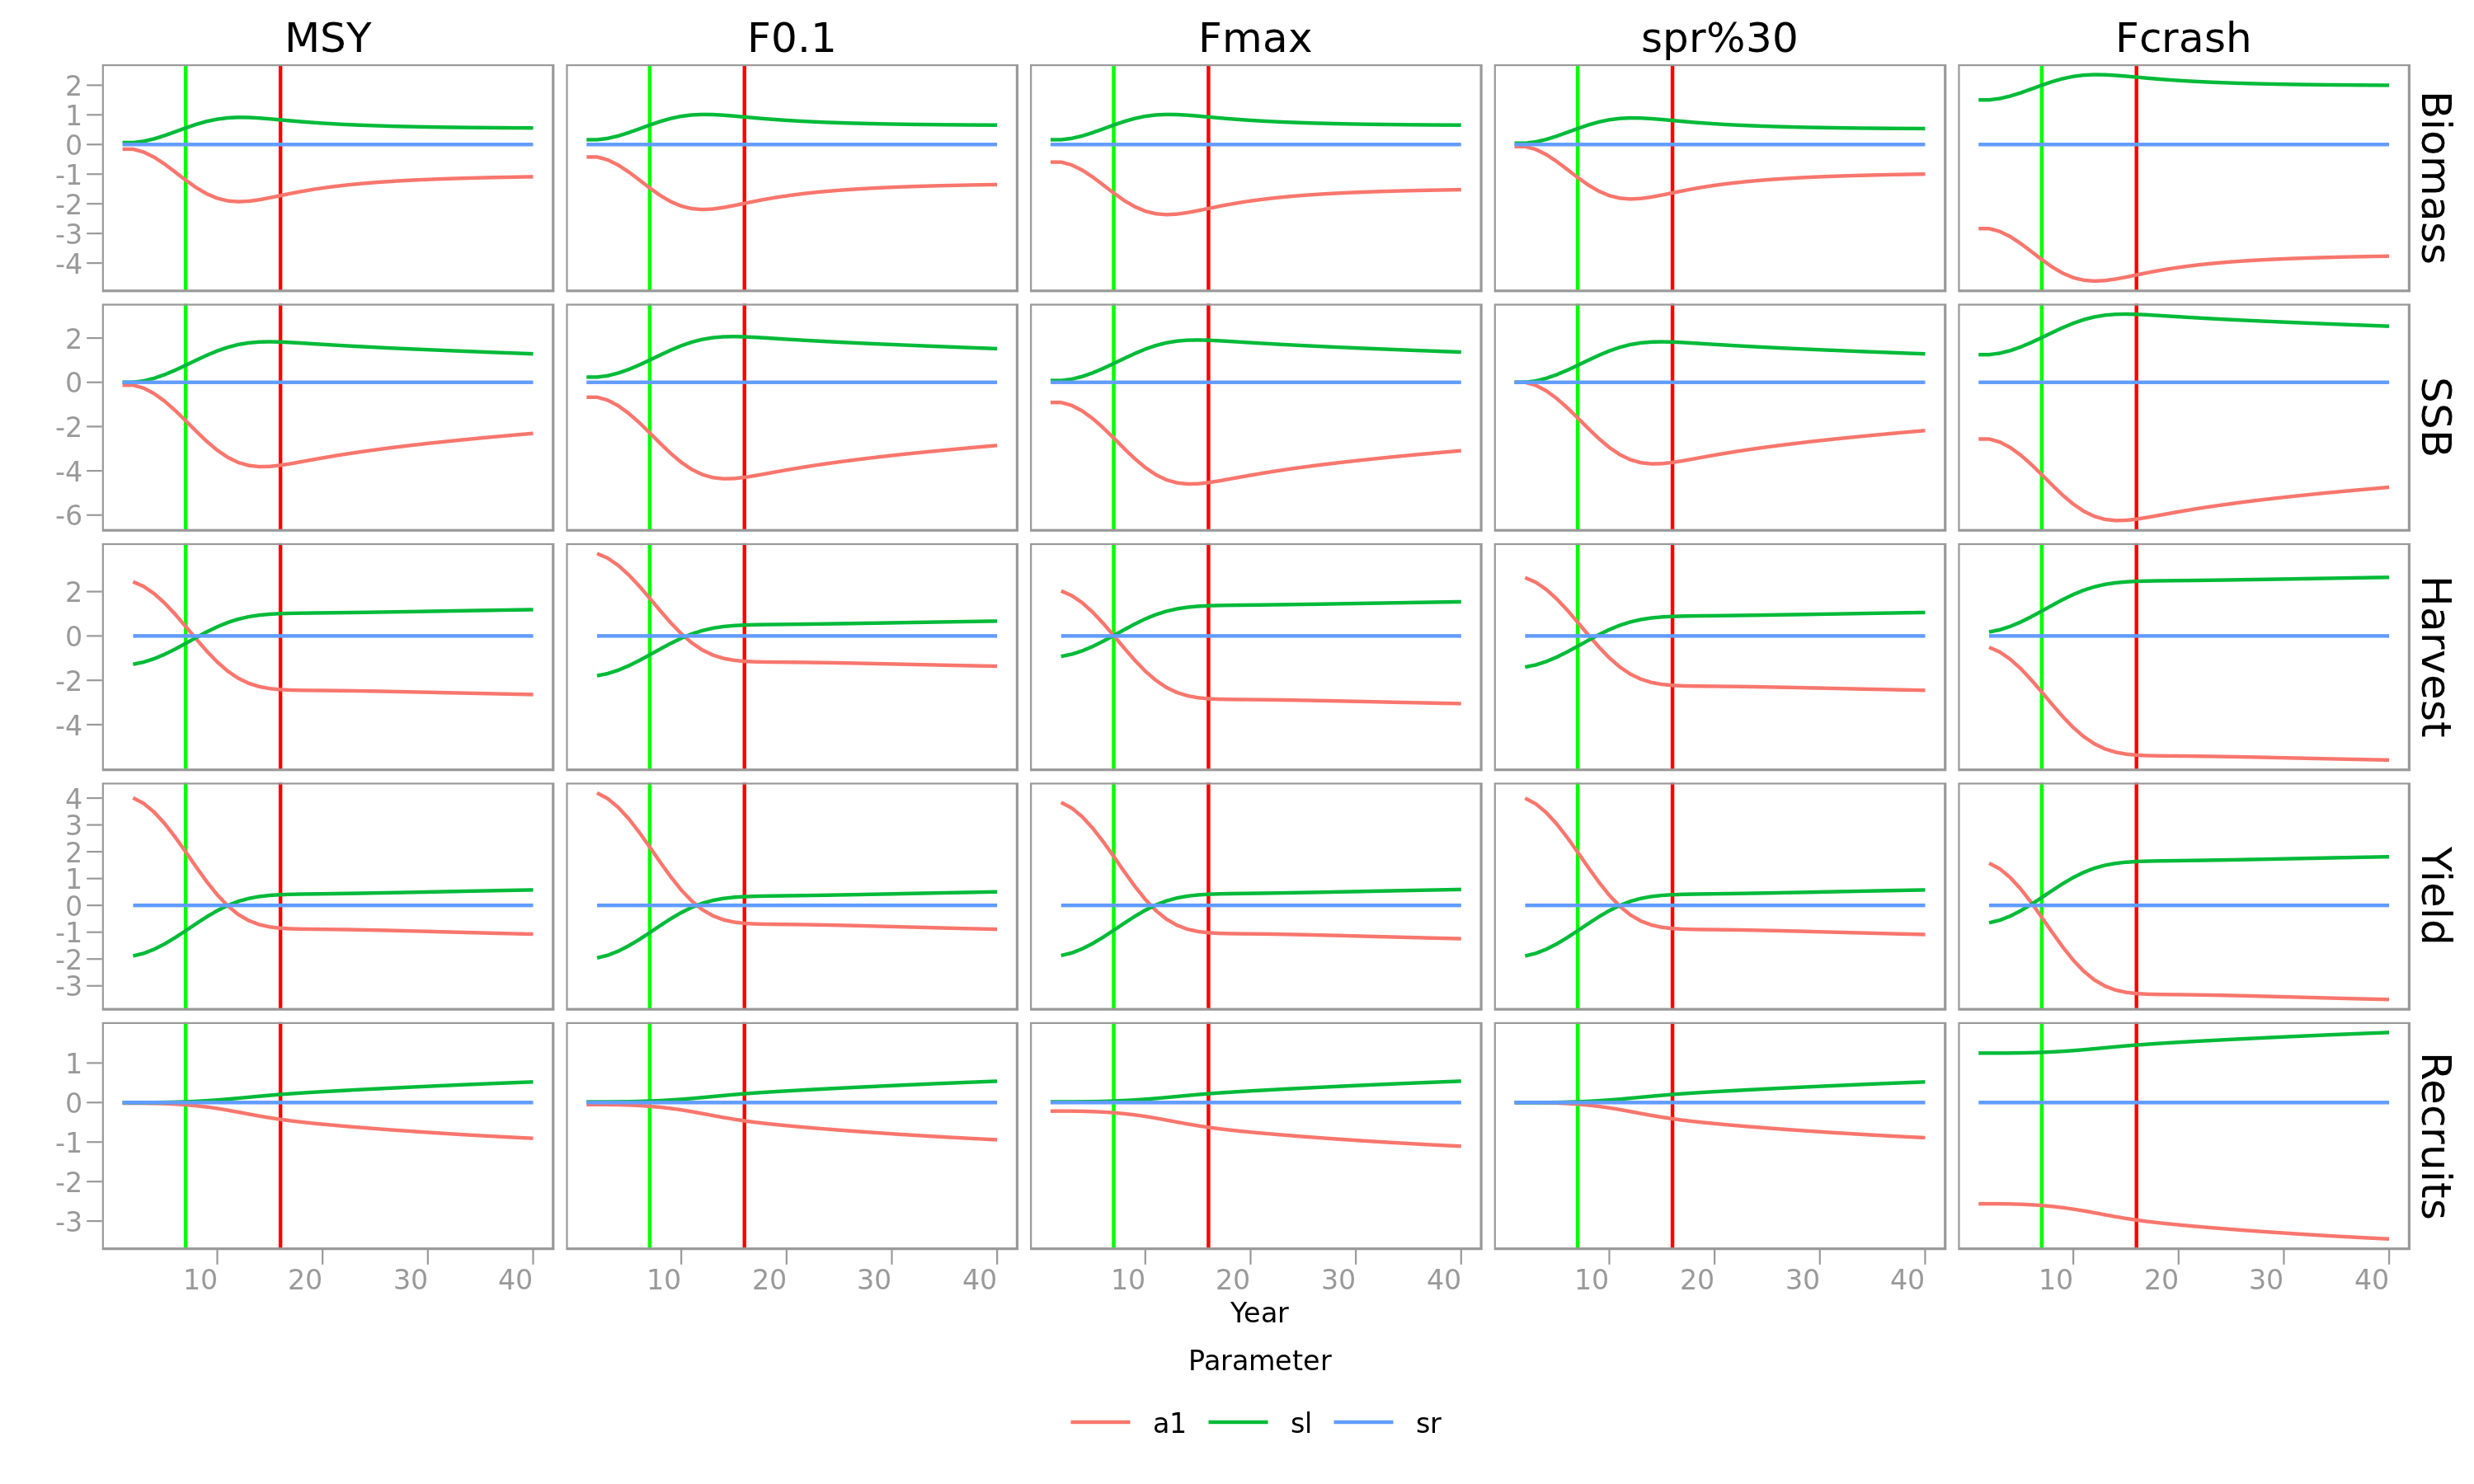
\includegraphics[height=4in, width=4in]{fig5.png}
\caption{\bf{Plots of elasticities for processess by year with respect to fishing mortality for  MSY, $F_{0.1}$ and $F_{crash}$ reference points.}}
\end{center}
\label{Figure_label_5}
\end{figure}

\begin{figure}[!ht]
\begin{center}
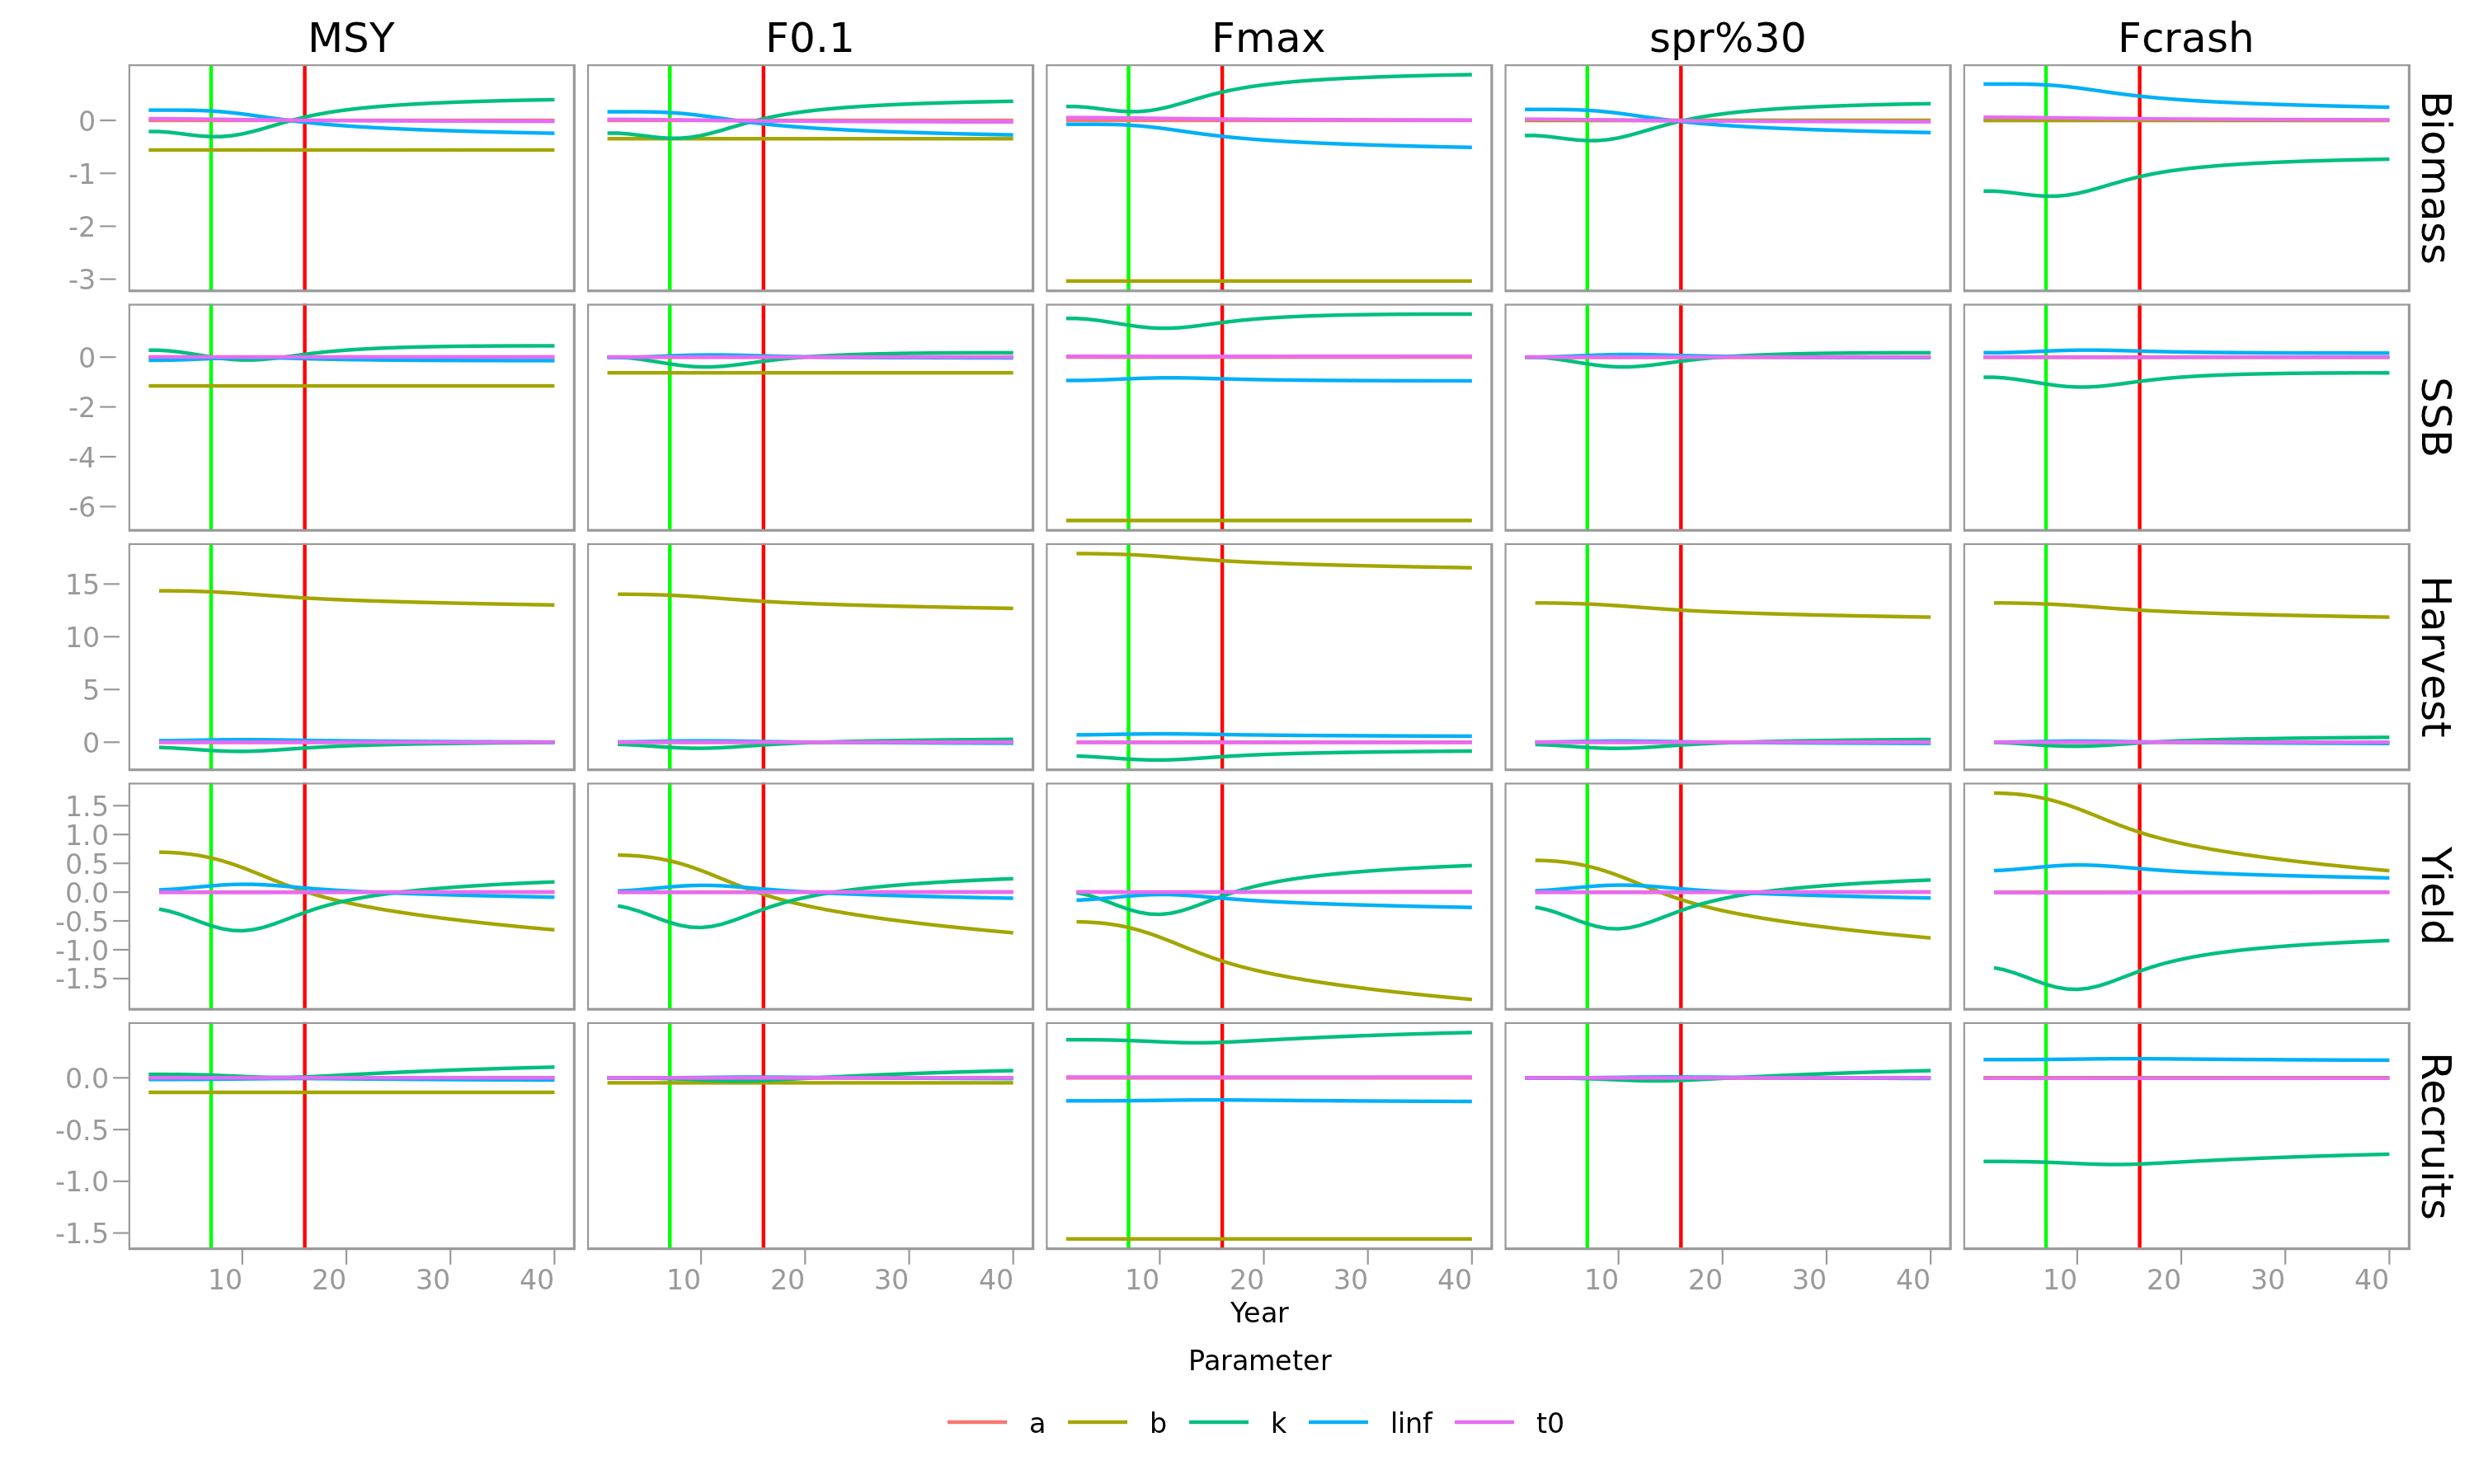
\includegraphics[height=4in, width=4in]{fig6.png}
\caption{\bf{Plots of elasticities for processess by year with respect to biomass for  MSY, $F_{0.1}$ and $F_{crash}$ reference points.}}
\end{center}
\label{Figure_label_6}
\end{figure}

\begin{figure}[!ht]
\begin{center}
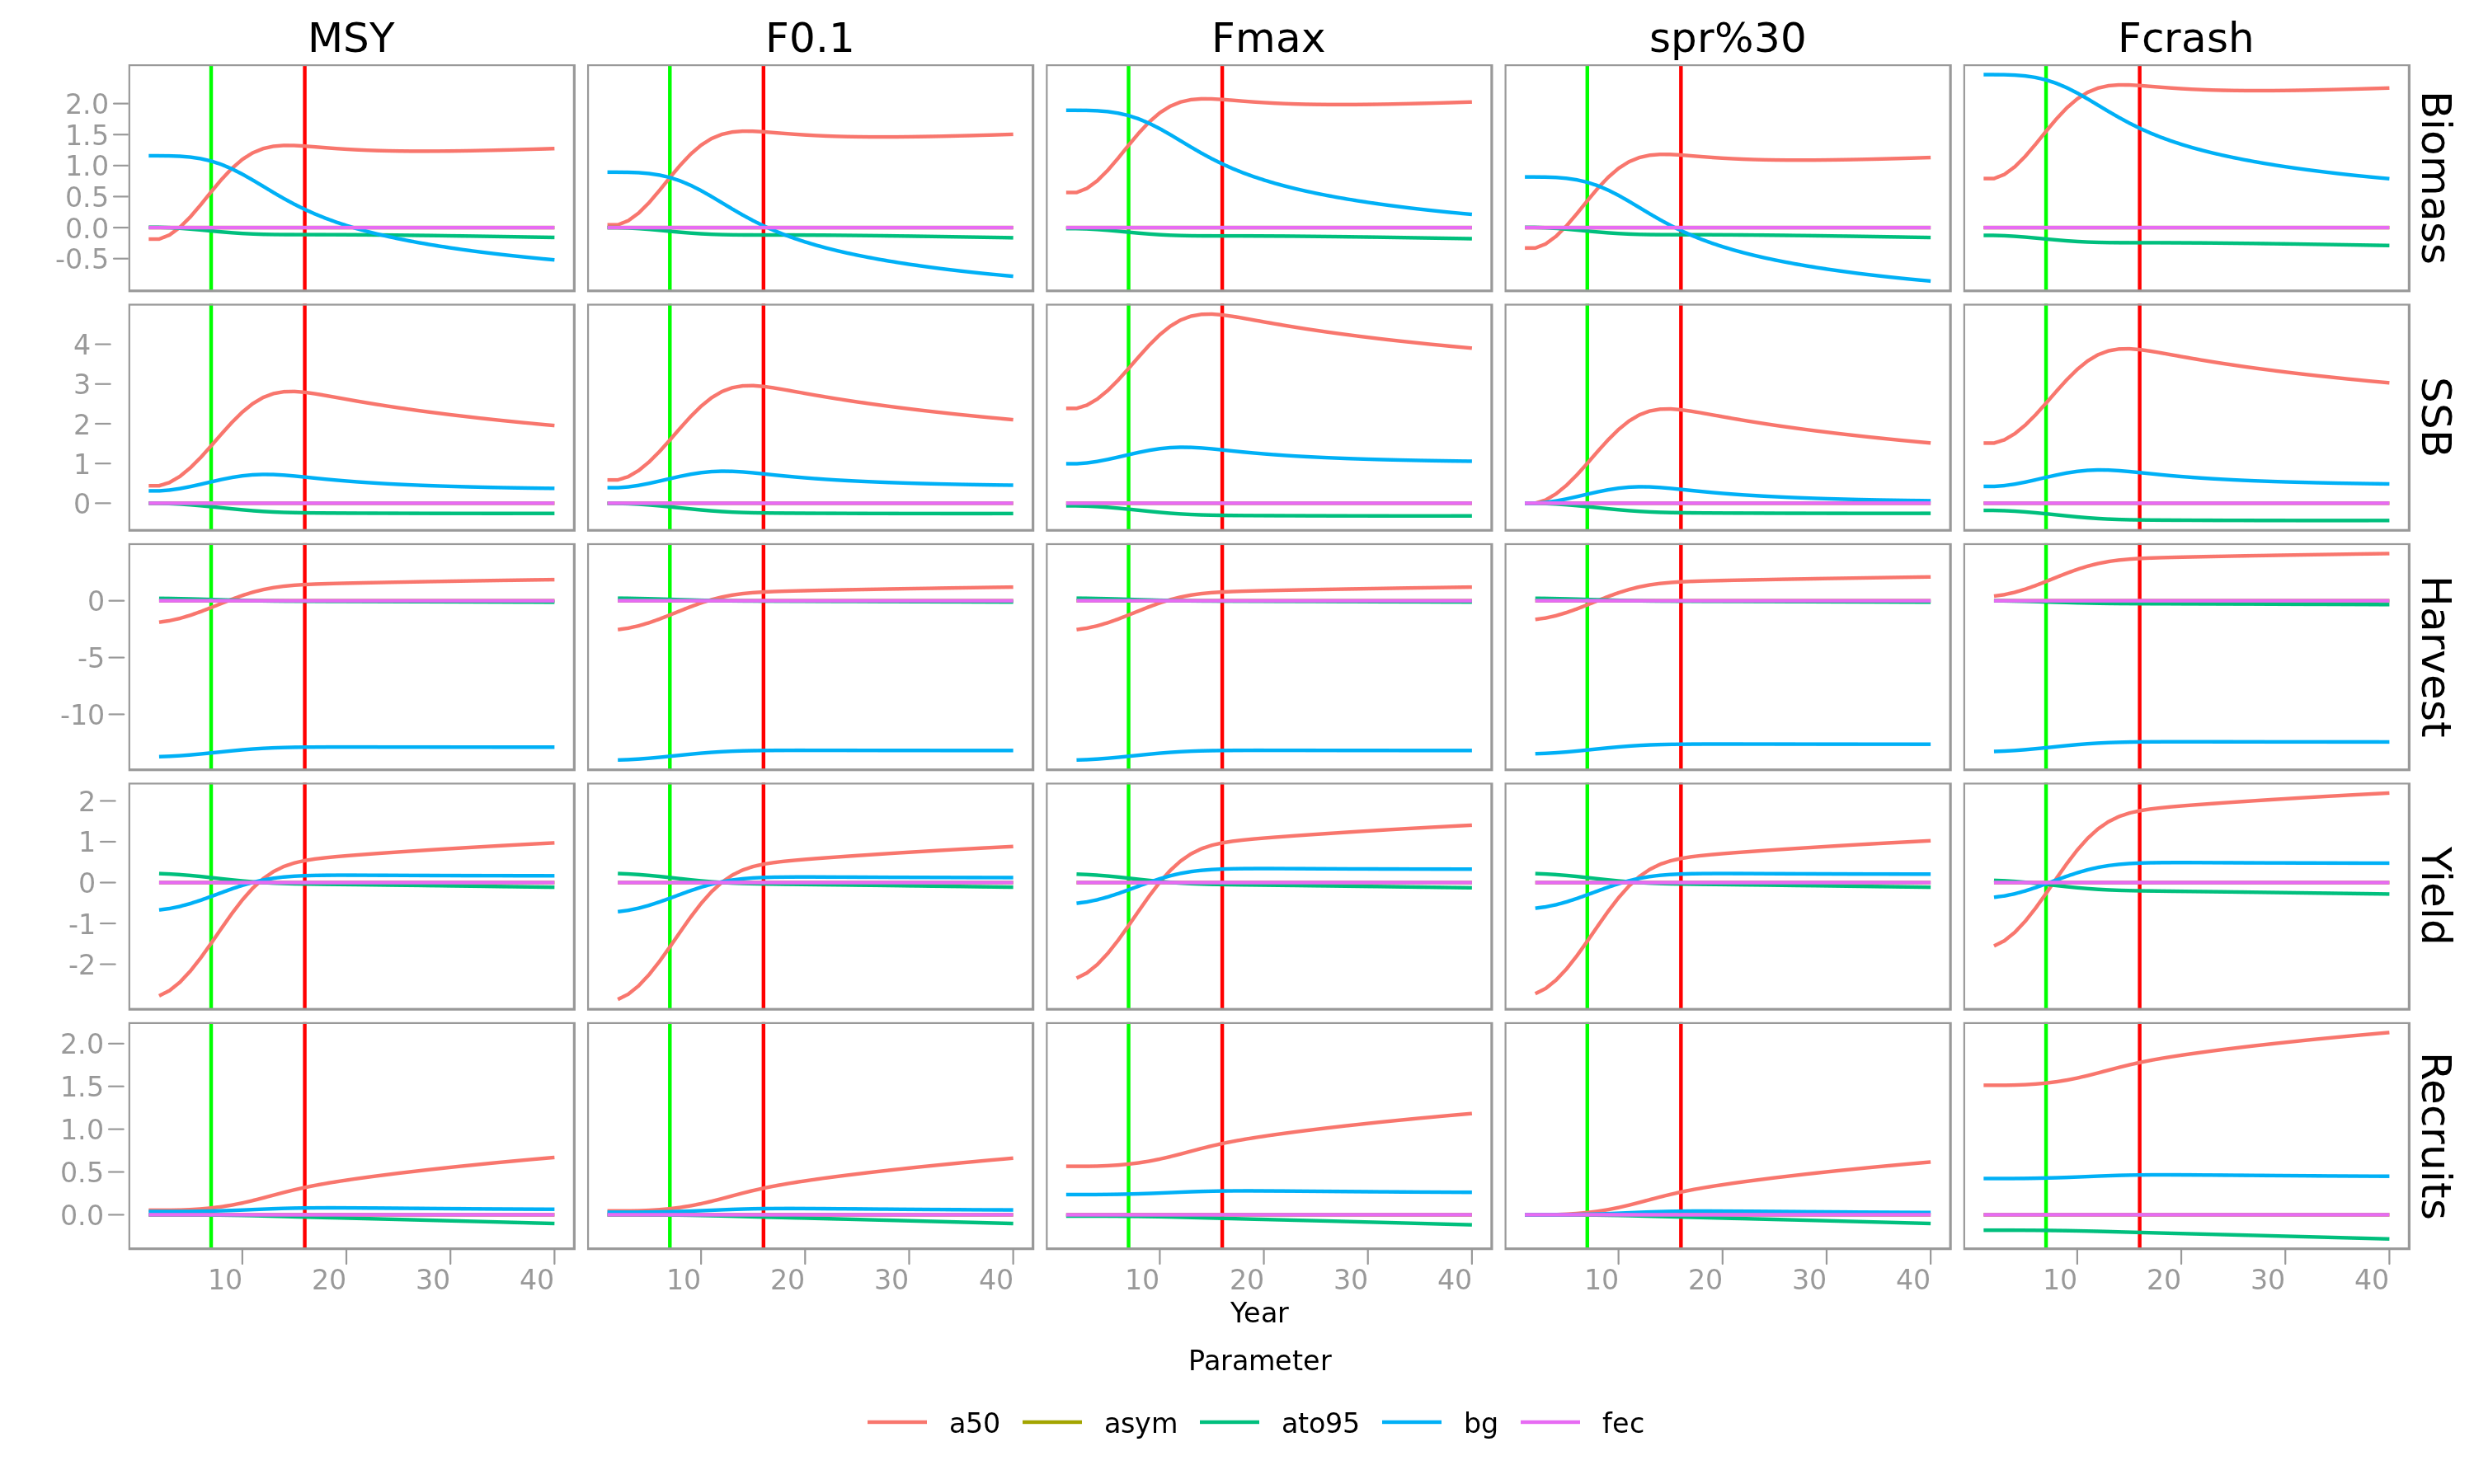
\includegraphics[height=4in, width=4in]{fig7.png}
\caption{\bf{Plots of elasticities for processess by year with respect to yield for  MSY, $F_{0.1}$ and $F_{crash}$ reference points.}}
\end{center}
\label{Figure_label_7}
\end{figure}


\section*{Tables}
%\begin{table}[!ht]
%\caption{
%\bf{Table title}}
%\begin{tabular}{|c|c|c|}
%table information
%\end{tabular}
%\begin{flushleft}Table caption
%\end{flushleft}
%\label{tab:label}
% \end{table}

\end{document}



